\subsection{Projection Matrix}
\label{Sec:Projection}
Wenn man sich einen Computerbildschirm anschaut, so stellt man fest, dass er eine zweidimensionale Oberfläche besitzt. 
Da aber die zu rendernde Szene dreidimensional ist, muss man diese Szene, bestehend aus mehreren dreidimensional angeordneten Grafik-Primitiven, auf diese zweidimensionale Oberfläche projizieren. Dafür verwendet man eine sogenannte \textit{Transformation}.
\todo[inline]{Keine Transformation}

Man kann sich das Ganze so vorstellen, dass eine simulierte ideale Version einer Loch-Kamera mit einem unendlich kleinen Loch verwendet wird. Dies bedeutet, dass alle Objekte scharf dargestellt werden. Da eine Lochkamera aber das Bild verkehrt herum abbildet, wird der Einfachheit halber die Bildebene vor dem Projektionszentrum abgebildet. Somit steht das Bild nun nicht mehr auf dem Kopf und muss nicht mehr invertiert werden. \cref{lochkamera}

Wenn wir uns nun einen Punkt $P(p_{x}, p_{y}, p_{z})$ in der Szene anschauen, so geht durch diesen vom Projektionszentrum bis zum projizierten Punkt auf dem Bildschirm $P'(p'_{x}, p'_{y}, p'_{z})$ eine Gerade. Mit dem Strahlensatz lässt sich nun aus $\dfrac{p'_{x}}{\mathnormal{f}} = \dfrac{p_{x}}{p_{z}} $ und $ \dfrac{p'_{y}}{\mathnormal{f}} = \dfrac{p_{y}}{p_{z}} $ die folgende Formel für Punkt $P$ bestimmen, die da lautet: $P'=(\mathnormal{f}\dfrac{p_{x}}{p_{z}}, \mathnormal{f}\dfrac{p_{y}}{p_{z}}, \mathnormal{f})$.
Nun kann die Projektion in einer Matrix abgebildet werden.

Weil $$\mathbf{P'}= \begin{pmatrix} p'_x \\ p'_y \\ p'_z \end{pmatrix}= \begin{pmatrix} f
\frac{p_x}{p_z}\\ f \frac{p_y}{p_z}\\ f \end{pmatrix} \in \mathbb{R}^3 \longmapsto \underline{\mathbf{P'}}= \begin{pmatrix}f \, p_x \\f \, p_y \\ f \, p_z\\
p_z\end{pmatrix} \in \mathbb{H}^3 $$
gilt:	


\begin{align}\mathbf{\underline{P'}} & =
	\begin{pmatrix}f \, p_x \\f \, p_y \\ f \, p_z\\ p_z\end{pmatrix}  = \begin{bmatrix} f & 0 & 0 & 0 \\ 0 & f & 0 & 0 \\ 0 & 0 & f & 0 \\ 0 & 0 & 1 & 0 \end{bmatrix} \begin{pmatrix}p_x \\p_y
		\\ p_z\\ 1 \end{pmatrix} \end{align}

Da die Projektion von OpenGL aber auf die negative Z-Achse ausgerichtet ist, gilt dementsprechend
\begin{align}\mathbf{\underline{P'}} & =
	\begin{pmatrix}f \, p_x \\f \, p_y \\ f \, p_z\\ -p_z\end{pmatrix}  = \begin{bmatrix} f & 0 & 0 & 0 \\ 0 & f & 0 & 0 \\ 0 & 0 & f & 0 \\ 0 & 0 & -1 & 0 \end{bmatrix} \begin{pmatrix}p_x \\p_y
		\\ p_z\\ 1\end{pmatrix} \end{align}

In der 3D-Computergrafik und somit auch in OpenGL verwendet man sogenannte \textit{Near-/ Far-Clipping} Ebenen, welche parallel zur Projektion (dem Bildschirm) stehen. Diese beiden Ebenen sind für die Begrenzung der Sicht gedacht. Alle Modelle/Punkte, die sich vor der \textit{Near-Clipping} Ebene befinden, sind zu nah. Dies heißt, dass sie nicht angezeigt werden sollen. Alle Modelle/Punkte, die sich vor der \textit{Far-Clipping} Ebene befinden, sind zu weit entfernt und werden ebenfalls nicht angezeigt. (Siehe \cref{nfplane}) Mathematisch kann man dies nun so umsetzen: für die \textit{Near-Clipping} Ebene hieße das $p_z=-z_n \quad$, dies entspricht $p'_z=-1$ . Die \textit{Far-Clipping} Ebene wäre mit $p_z=-z_f \quad$ definiert, was auch als $p'_z=1$ geschrieben werden kann.

Zuerst nehmen wir uns die Parameter $a$ und $b$ in unsere bisherige Transformations-Matrix. 
\todo[inline]{TODO!}
%\url{http://www.mathematik.uni-marburg.de/~thormae/lectures/graphics1/graphics_6_1_ger_web.html#15}

\begin{figure}
	\centering
	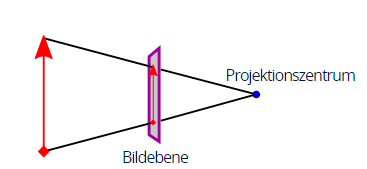
\includegraphics[scale=0.7]{02theorie/Lochkamera.png}
	Quelle: \url{http://www.mathematik.uni-marburg.de/~thormae/lectures/graphics1/graphics_6_1_ger_web.html#10}	
	11.01.2017
	\caption{Lochkamera in der Grafikprogrammierung}\label{lochkamera}
\end{figure}

\begin{figure}
	\centering
	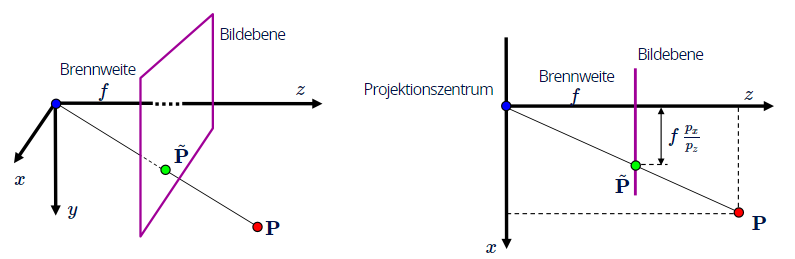
\includegraphics[scale=0.7]{02theorie/perspektivischeprojektion.png}
	Quelle: \url{http://www.mathematik.uni-marburg.de/~thormae/lectures/graphics1/graphics_6_1_ger_web.html#11}	
	11.01.2017
	\caption{Perspektivische Projektion}\label{perspproj}
\end{figure}

\begin{figure}
	\centering
	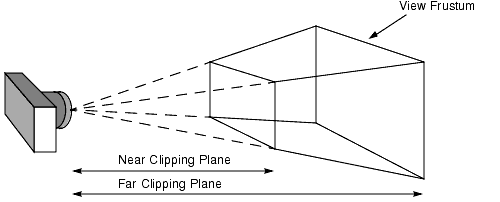
\includegraphics[scale=0.7]{02theorie/ViewModel11.png}
	Quelle: \url{http://download.java.net/media/java3d/javadoc/1.4.0/javax/media/j3d/doc-files/ViewModel11.gif}	
	14.01.2017
	\caption{Near-/Far-Clipping Plane}\label{nfplane}
\end{figure}
